\chapter{电力系统脆弱性分析及结构与状态脆弱性研究}
\label{cha:theory}

\section{引言}
\label{sec:index3}

近年来,脆弱性一直是电力系统领域研究的热点。对于电力系统而言,脆弱性的概念目前还没有清晰明确的定义。目前大多数学者认为,电力系统脆弱性是系统本身固有的属性,
在正常运行状态下不会显现。由于电力系统内部结构的复杂性,加之对外部环境的依赖性,在外界扰动或内部结构参数作用下,电力系统的性能参数将会偏离正常范围,影响其电能
质量,因此分析电力系统的脆弱性很有研究意义。

本章将电力系统的脆弱性从两个方面进行展开分析,即结构和状态两个方面,首先从系统整体的脆弱性分析与描述入手,得到清晰合理的电力系统脆弱性本质概念和数学描述;
在此基础上,分别从结构和状态两个方面对系统脆弱性进行分析,在结构方面,主要基于复杂网络和$PageRank$理论进行分析,其脆弱性研究专注于系统受影响的程度;在状态方面,
主要基于蒙特卡洛和概率潮流方法进行分析,其脆弱性研究侧重于抗干扰能力。

\section{电力系统脆弱性分析与描述}
\label{sec:defina}

本节首先对电力系统的稳定性、可靠性以及鲁棒性进行研究分析;在此基础上,结合电力系统脆弱性的特征,得到较为明确的电力系统脆弱性本质概念;进而对电力系统的脆性过程
进行分析,并给出电力系统脆弱性的数学描述。


\subsection{电力系统稳定性、可靠性、鲁棒性的区别与联系}
\label{sec:network}

对于电力系统而言,在进行电力系统脆弱性研究分析之前,有必要明确电力系统脆弱性的概念,不可避免要涉及到系统的稳定性、可靠性以及鲁棒性。这些系统性能概念的提出是为解决
不同的工程实际问题,然而这些概念本身又有相互重叠的部分,因此需要分析电力系统稳定性、可靠性、鲁棒性的概念本质,找出它们之间的区别与联系。并进一步结合电力系统脆弱性的特征,
得到较为明确的电力系统脆弱性概念。

$(1)$稳定性

电力系统的稳定性是当电力系统受到外界扰动时发生的稳定性问题。主要表现在两个方面。当电力系统受到瞬态干扰时,电力系统会偏离原平衡状态,产生偏差,在瞬态扰动消失后,电力
系统可以恢复到原平衡状态;另一方面,当电力系统受到永久性扰动时,如电力系统的节点或线路遭到破坏时,电力系统在经历一个过渡过程后,偏离原平衡状态,达到一种新的平衡状态。
通过上述的定义,电力系统稳定性主要的关注点在于扰动消失后,系统能否恢复到原平衡状态,以及在永久性扰动情况下,系统能否达到新的平衡状态,实现系统稳定运行。

$(2)$可靠性

广义上来说,可靠性是评价元件、产品、系统在一定时间及一定条件下无故障运行的能力或可能性。电力系统的可靠性是指元件、设备或系统在预定时间内,在规定条件下执行规定功能的能力
\cite{refs62}。具体来讲,对于用户而言,电力系统的可靠性是指系统向用户长时间不间断持续提供满足质量要求的电能的能力。这种能力可以通过可靠度、失效率、平均无故障间隔等来
评价。由以上定义可知,电力系统的可靠性主要的关注点在于系统在规定时间内,在规定参数下工作的能力。

$(3)$鲁棒性

鲁棒性一词是原先统计学中的一个专业术语,20世纪70年代才开始在控制理论的研究中流行起来,用来表征控制系统对特征或参数扰动的不敏感性\cite{refs63}。所谓控制系统的鲁棒性是指系统在
自身内部模型不确定性扰动及外部摄动的影响下,系统某个性能指标保持不变的能力。在电力系统中,电力系统的鲁棒性是指系统受到外界扰动或内部自身故障后,系统中绝大部分节点或线路的状
态值保持在稳定裕度范围内变化的能力。也就是说电网中绝大部分节点仍然保持连通。电力系统鲁棒性的主要关注点在于电力系统的抗干扰能力。

通过研究分析系统的稳定性、可靠性以及鲁棒性的定义来看,这三个性能指标的区别如下表所示。

\begin{table}[H]
\centering
\caption{稳定性、可靠性、鲁棒性的区别}
\label{tab:chap3:deference}
\begin{tabular}{C{3cm}C{3cm}C{3cm}C{3cm}}
\toprule
\textbf{系统性能} & \textbf{稳定性} & \textbf{可靠性} & \textbf{鲁棒性}\\
    \midrule
    产生原因       &外部扰动           &外部扰动、内部参数变化         &外部扰动、局部故障\\
    主要关注点     &系统能否回到原平衡状态或能否达到新的平衡状态 
                                          &系统在规定时间和参数下的满足性能运行指标的能力 
                                                                        &系统的抗干扰能力\\
\bottomrule
\end{tabular}
\end{table}

电力系统在稳定性、可靠性和鲁棒性的定义可知,三者的主要关注点上略有不同,如上表所示,然而在产生原因、分析思路和内在概念上,又有着内在的联系。

稳定性是电力系统的基本保障。可靠性是在稳定性的基础上,针对具体的性能指标,可靠性强调的是在规定时间保持规定指标要求运行的能力。鲁棒性是在稳定性的基础上,研究在外界扰动或发生
局部故障后,系统性能参数保持在稳定裕度范围内的能力。

与鲁棒性概念有一点类似,不同之处在于,一是脆弱性是电力系统固有的属性,任何一个电力系统都存在脆弱性,系统正常运行的情况下,不会显现;二是其耐受程度不但包括系统抗干扰的能力,还
包括系统受影响的程度;三是电力系统的脆弱性包括结构脆弱性和状态脆弱性两个方面。电力系统可靠性概念可为研究系统状态脆弱性指标提供借鉴的思路。


\subsection{电力系统脆弱性的本质及脆弱过程分析}
\label{sec:network}

复杂系统的脆弱性是指:对于一个复杂系统$S$,存在一个子系统$S_i$,对环境有强烈的敏感性,当$S_i$受到内、外因素(包括信息、物质流等因素)的扰动或攻击产生崩溃时,会使其他部分或子系统也产生崩溃,
进而导致整个复杂系统崩溃\cite{refs61}。对于复杂系统所具有的这一特性称之为复杂系统的脆弱性。

经过上一节对电力系统性能的研究分析后,结合复杂系统脆性理论,对电力系统脆弱性的本质概念进行如下研究探讨。

电力系统作为复杂系统中的一种典型系统,其脆弱性是系统本身固有的一种属性,在正常运行和工作状态下不会显现。在电力系统中,每个子系统或元件是相互关联的,当子系统或单个元件由于外界
扰动或自身参数变化而使正常运行状态改变时,会导致系统承受不确定性因素的能力变差,这种特性即为系统的脆弱性。它表现的是系统对外界扰动或自身参数变化的耐受程度。其耐受程度由两个
方面的体现,一是系统受影响的程度;二是系统抗干扰的能力。

电力系统耐受程度可通过系统性能指标进行分析,当外部扰动或内部参数改变时,系统的性能指标在稳定裕度范围内变化,说明系统的耐受程度高,系统脆弱性差,反之,系统性能参数超出稳定裕度范围,
系统性能变差,系统脆弱性强。

按研究角度的不同,将电力系统的脆弱性分为结构脆弱性和状态脆弱性。结构脆弱性研究的是电力系统中某个元件在网络拓扑的重要程度;状态脆弱性则研究的是电力系统各状态变量偏离正常运行状态
及距离临界状态的程度。

脆弱过程分析:????

\subsection{电力系统脆弱性的数学描述}
\label{sec:describtion}

通过对电力系统脆弱性本质概念的分析研究可以得出,对于电力系统而言,系统性能变化的主要原因是外部扰动对系统元件的影响以及元件内部结构参数的变化,即脆弱源。脆弱源作用于脆弱环节,使得
系统脆弱性凸显,系统性能变差。

设系统$S$由$n$个元件$C_i$组成,且$C_i$的状态用$x_i$表示,$x_i \in X \subset R^m$。如果存在一个元件$C_b$,当其结构或状态发生变化,使得$x_b \to x_B$,有
\begin{equation}
  \lim _{g\left(x_{0}\right) \rightarrow G\left(x_{s}\right)} \delta(s) \neq \delta\left(s^{-}\right)
  \end{equation}
 
式中,$\delta\left(s^{-}\right)$为系统初始稳态的性能指标,$B$为元件$C_B$的不稳定域,$G\left(x_{B}\right)$为$C_B$不稳定域的阈值函数,$g(x_b)$是衡量$C_b$元件的性能指标,
$\delta\left(s\right)$为当前系统$S$的性能指标。

复杂系统是由元件、关系、环境组成的,元件在电力系统中对应着母线节点和线路,关系对应着节点之间的连接情况和潮流分布流向,环境对应的是一切影响电力系统结构或状态参数原因的集合。研究电
力系统的脆弱性,主要就是研究在不确定的环境中各元件之间、元件与整体之间、元件与环境之间以及整体与环境之间的内在关系,本文的主要研究方向是电力系统的节点或线路受到不确定因素影响后结
构或状态发生变化,对其他元件和整个系统产生的影响。

可以看出,系统脆弱性的数学描述和定义主要在于元件的存在性对于整个电力系统的影响,即存在能够引起整个系统性能改变的元件,量化系统中的元件对整个系统的重要程度,以及如何识别出这样的元件
是电力系统脆弱性研究的一个重要方向,通过加强对脆弱环节的重点保护和电网拓扑的优化改进,从而为预防大规模停电事故和连锁故障的发生提供了参考方向。


\section{电力系统结构脆弱性研究}
\label{sec:construction}

电力系统的结构主要是指由发电节点、负荷节点和传输线路组成的网络拓扑。拓扑结构是电能传输和系统性能的基础,它决定了电能是否能够被安全、可靠、有效地从发电节点传输到负荷节点。当电力系统
拓扑结构保持完整时,是保证电力系统稳定可靠运行的基础。但是,受外界环境的干扰,人为因素和保护设备内部故障等原因的影响,拓扑结构的完整性会受到破坏,导致电力系统无法安全可靠运行,甚至
崩溃。因此,有必要分析各个节点在网络拓扑的重要程度,进而加强对重要节点的防范和预先保护,对电力系统的稳定、高效、可靠运行有重大意义。

\subsection{电力系统结构脆弱性定义与数学描述}
\label{sec:network}

电力系统的结构脆弱性是指电力拓扑结构中节点或线路由于外界或内部因素的影响下,导致节点或线路发生故障断开后,电网保持其连通性和维持基本稳定运行状态的能力,即保持拓扑结构完整的能力。

在电网拓扑结构方面可选取一定的评估指标,来考察某一单元或某些单元退出后系统的耐受程度——系统受影响的程度。对系统结构影响程度大的节点或线路,说明其对网络拓扑结构的完整性贡献程度高,
对于这样的节点或线路称为系统结构的脆弱点。因此,可以认为对电力系统拓扑结构影响越大的节点或线路,其脆弱性程度越高。

结构脆弱性研究的是电力系统中某个单元在网络拓扑的重要程度。在电力系统拓扑结构方面,从不同方面研究得到的结构脆弱性的指标描述不同,每个方面都有其结构重要性指标来衡量一个元件$i$在系统
中的重要程度,其数学描述如下:
\begin{equation}
  A(i)=\sum_{j\in F(i)}{k(i,j)}
  \end{equation}

$F(i)$为元件$i$有关联的元件的集合,$k(i,j)$为从不同角度考虑得到的结构脆弱性表达式,表示$i$和$j$在拓扑结构上的联结程度。

% 将$A_l(i)=\sum_{j \in F(i)}{k_l(i,j)}$定义为从某一方面考虑的结构脆弱性描述,那么从各个方面考虑的结构脆弱性数学描述定义为结构矩阵$Z$,$Z=[A_1,A_2,A_3\cdots A_n]]$于是结构脆弱性
% 矩阵的数学描述为


\subsection{基于复杂网络的结构脆弱性研究}
\label{sec:network}


\subsection{基于$PageRank$的结构脆弱性研究}
\label{sec:pagerank}

$PageRank$最早是被用来作为互联网网页结构的模型,并且对所有网页的重要度进行量化评估的一种算法\cite{PR1,PR2,PR3}。在众多计算互联网网页的相关性的算法中,$PageRank$是名气最大,且最早被谷歌浏览器采用的。$PageRank$的基本思想是一个网页的重要性依赖于所有链接向它的其他网页。比如,网页$i$有链接指向网页$j$,如果有很多其他网页有链接指向网页$j$,那么我们认为,网页$j$是非常重要的。另一方面,若只有一个网页有链接指向网页$j$,但是这个网页是一个权威性很高的网址,如谷歌,百度等网页,我们认为网页$j$也非常重要,因为由受欢迎、权威的网页指向它,这份重要性将会传递下来。

电网中,每条支路上的潮流是有确定的方向的,所以可以被视为一个有向图。其中,每个母线节点被视为一个网页,母线节点之间的电气连接被视为网页中的超链接,根据电流的方向决定超链接的方向。互联网与电网的$PageRank$的拓扑模型比较如表~\ref{tab:PRComparision}。已有的研究中,大多学者在$PageRank$模型的网页出链的处理上采用均分的思想\cite{PRNET},本文在综合考虑潮流能量对结构的影响下,认为出链是按照实际的潮流的比重进行分配的。

即按照网页的超链接可以传递重要性的思想,假设$A$节点拥有~3~个出链,它会分别按照视在功率的比例分别传递给所指向的$B$、$C$、$D$三个节点,按照能量的分布作为权重。根据重要性传递规则,可以得到能量转移矩阵$A$。对于没有出链的节点,则按照$PageRank$的算法,认为该节点对所有节点都出链,从而解决终止点的问题。因为电网的潮流能量分布中不存在自己指向自己的连接,故不存在陷阱问题,因此不予考虑。
\begin{table}[htb]
  \centering
  \caption{互联网与电网的$PageRank$拓扑模型比较}
  \label{tab:PRComparision}
    \begin{tabular}{C{4.5cm}C{4.5cm}C{4cm}}
      \toprule
      互联网 & 电网 & $PageRank$拓扑 \\
      \midrule
      网页 & 母线 & 节点\\
      超链接 & 输电支路 & 有向边\\
      指向该网页的网页数目 & 母线进线数目 & 入度\\
      该网页指向的网页数目 & 母线出线数目 & 出度\\
      \bottomrule
    \end{tabular}
\end{table}

$PageRank$算法应用于电网拓扑的具体步骤为:

$(1)$假定初始服从均匀分布,即每个母线节点的重要性都是相同的,即对于一个一共有$n$个节点的系统而言,赋予每个网页初始相同的$PR$值,一般都为1。

$(2)$根据电网的实际潮流计算每条连接上的视在功率得到能量分布权重的矩阵P,再根据公式\ref{equ:chap3:Index3}得到能量转移矩阵A。

$(3)$迭代计算,由于每个超链接的存在都会增加对应网页的$PR$值,所以通过考虑潮流连接、能量转移情况对各个母线节点的$PR$值进行迭代更新。

$(4)$最后,经过若干次的迭代后,各个母线节点的$PR$值会趋于一个稳定的值。
\begin{equation}
\label{equ:chap3:Index3}
PR(p_i)=\frac{1-q}{N}+q\sum\limits_{p_j\in\mathbf{M_{p_i}}}{\frac{PR(p_j)}{L(p_j)}}
\end{equation}

式~(\ref{equ:chap3:Index3})中,$p_i$是被计算的节点,$M_{p_i}$是节点$p_i$的入链节点集合,$L(p_j)$是节点$p_j$的出链数目,$N$是节点总数目。$q$为阻尼系数,一般取~0.85~,引入该参数是为了解决出链为零的节点在模型计算中带来的问题,代表了当前的母线节点没有遭到破坏正常运行的概率。$1-q$则代表了节点遭到意外破坏退出运行的概率。从公式中可以看出,$p_i$节点的$PR$值与和它相连的$p_j$节点的$PR$值有关,其值越大,且$p_j$节点的出链越少,$p_i$节点的$PR$值越大。其计算流程图如下:
\begin{figure}[H] % use float package if you want it here
  \centering
  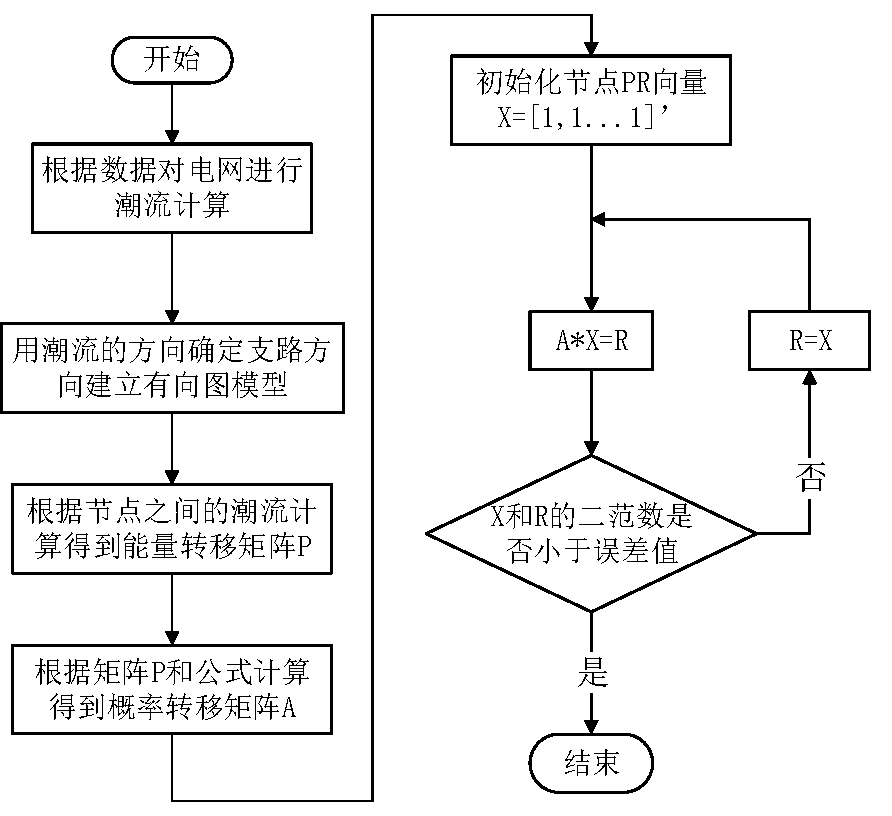
\includegraphics[height=8.4cm]{PRprocess.pdf}
  \caption{$PangRank$计算流程}
  \label{fig:PRPro}
\end{figure}

由图可知在$PageRank$在计算中,考虑更多的是节点的重要性在拓扑中的传递性。即通过反复迭代,确保所有节点的$PageRank$值在整个拓扑的重要性分配中趋于稳定,误差达到最小。$PR$值代表了节点在网络中的重要程度,$PR$值越高,节点越重要。

\subsection{模型比较与案例分析}
基于前面的研究可知,对电力系统的拓扑建模有两种不同的角度。不考虑潮流的方向,关注支路的重要性可将系统视为一个加权无向图。反之,考虑潮流的方向,衡量出入链对结构的影响可将系统视为一个有向图。复杂网络的电气介数更多关注的是支路上的潮流分布对拓扑重要性影响,而$PageRank$算法则更多关注的是有向的连接关系对拓扑重要性的影响。本节以$IEEE14$数据集为例,分别用以上的两种方式建模。该电网拓扑原理图如下:
\begin{figure}[H] % use float package if you want it here
  \centering
  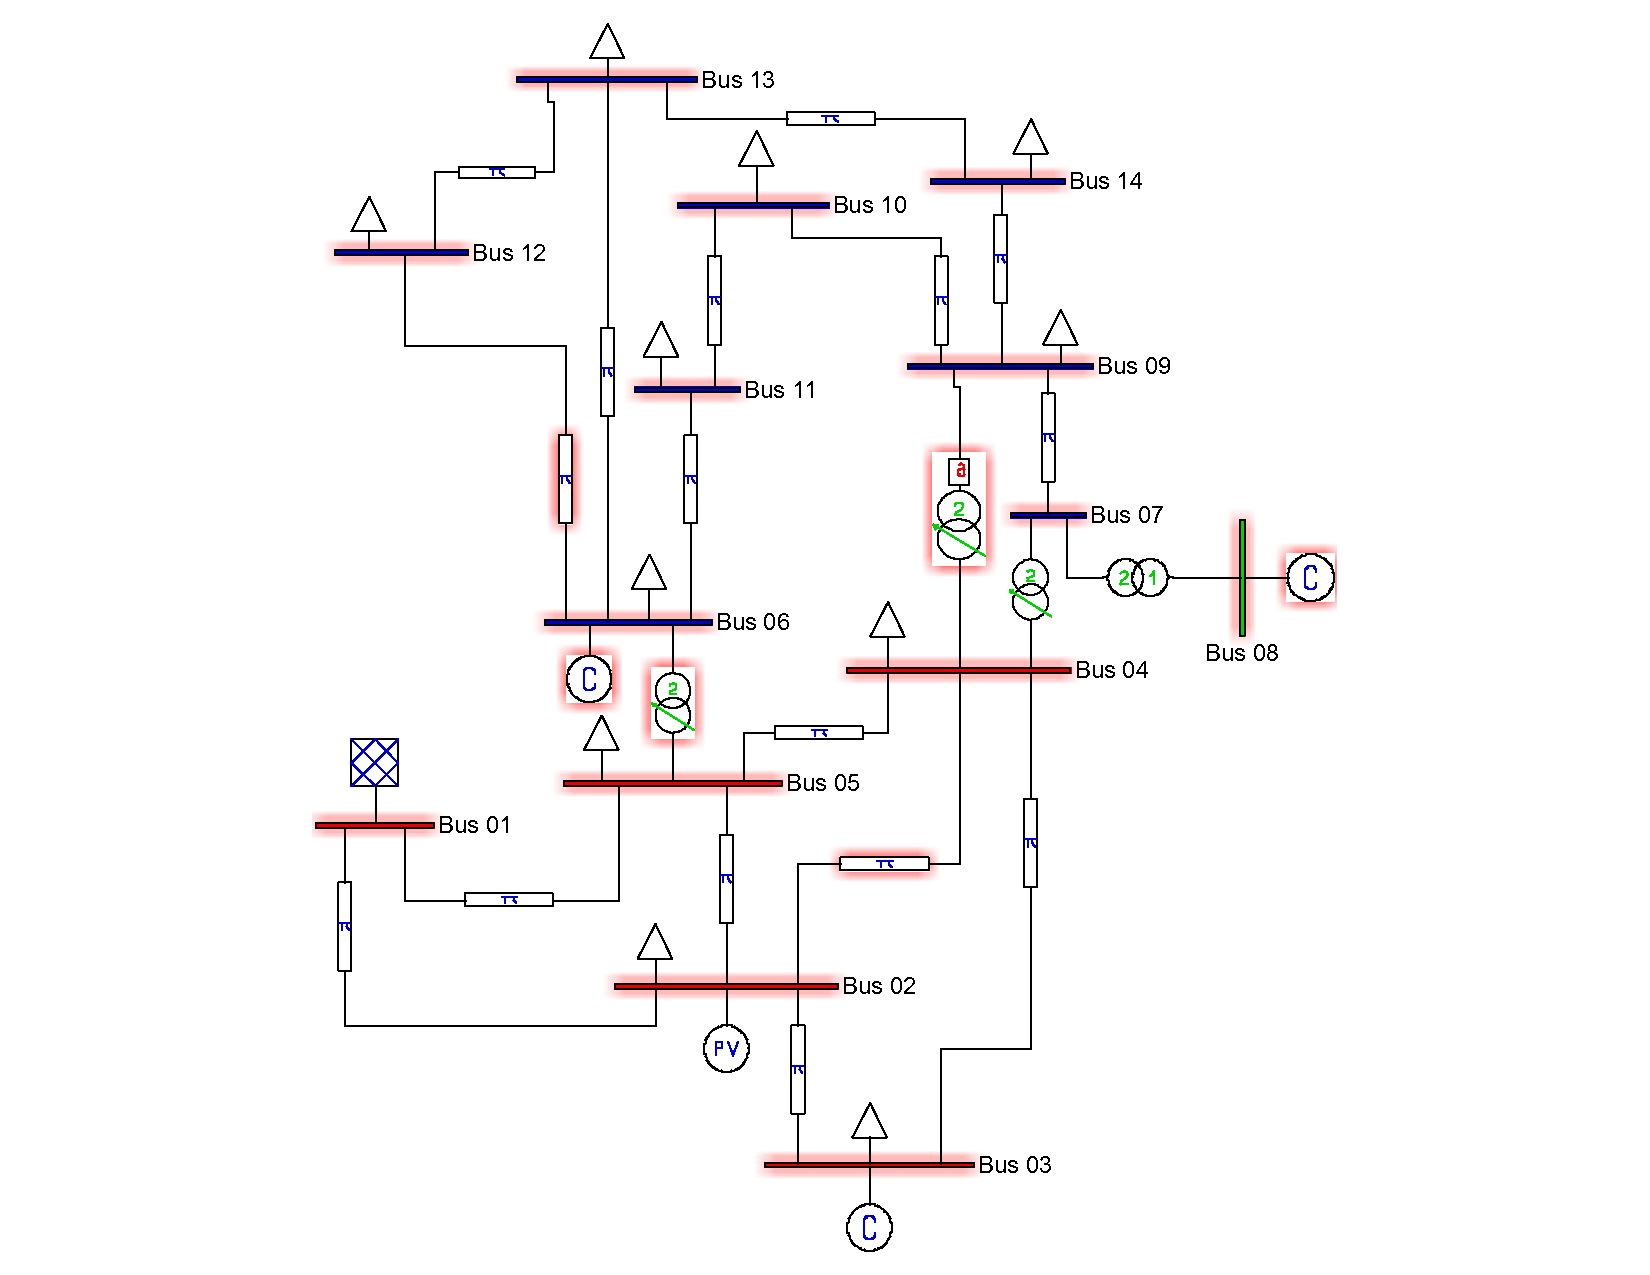
\includegraphics[height=13cm]{IEEE14.pdf}
  \caption{$IEEE14$电网拓扑原理图}
  \label{fig:fundement14}
\end{figure}

针对该拓扑,复杂网络的建模将其等效为一个无向图如图\ref{fig:model1},图中按照支路电气介数的大小等比例加粗了图的边,再根据图中的流程\ref{fig:nodeBetweenPro}最终计算得到各个节点的电气介数。电气介数计算的过程中,节点的电气介数直接受支路的电气介数影响。而支路的电气介数计算突出的是支路结构对能量分布的影响,能量分布越大的支路其电气介数也相应的越高。而$PangRank$的建模则将其等效为一个有向图如图\ref{fig:model2},再根据图\ref{fig:PRPro}最终计算得到各个节点的$PR$值。$PangRank$计算的过程中,突出的是拓扑的出入链的重要性。对于该模型,其迭代过程在能量转移矩阵的作用下完成,而入链累计度越高的点的$PangRank$越高。$PangRank$衡量了拓扑节点在能量转移中所起的作用。
\begin{figure}[H]
\begin{minipage}{0.48\textwidth}
  \centering
  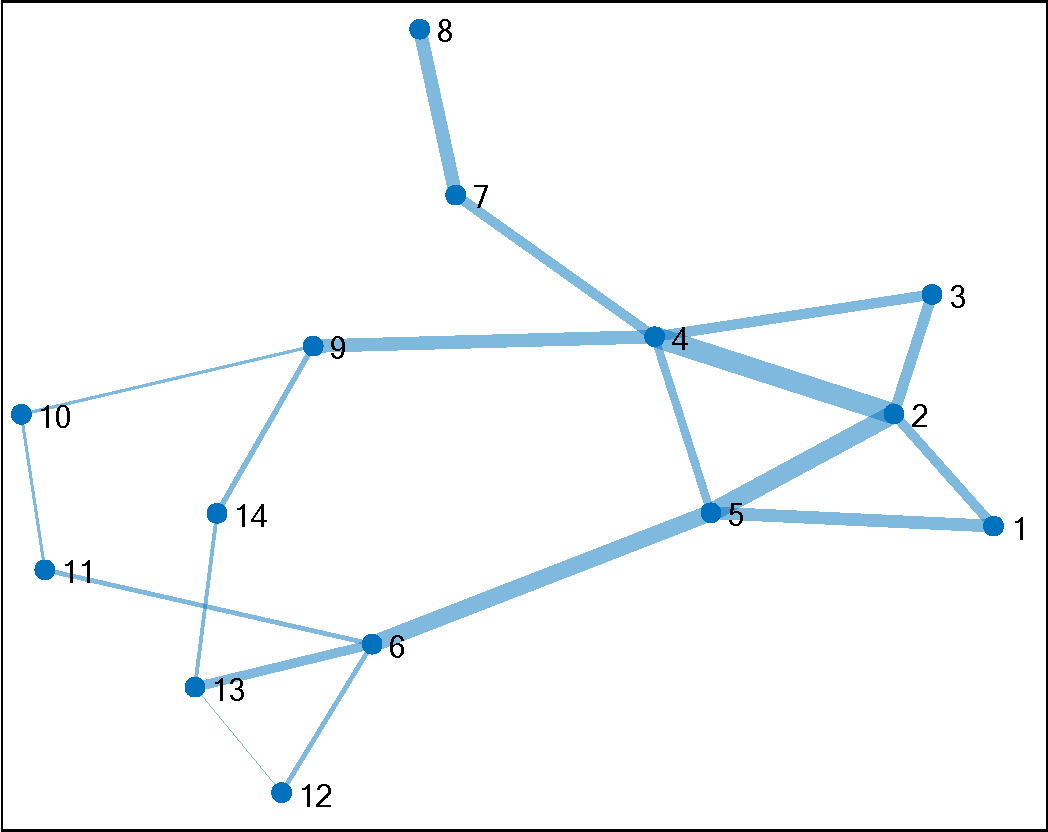
\includegraphics[height=5.8cm]{graph14.pdf}
  \caption{基于复杂网络的拓扑建模}
  \label{fig:model1}
\end{minipage}\hfill
\begin{minipage}{0.48\textwidth}
  \centering
  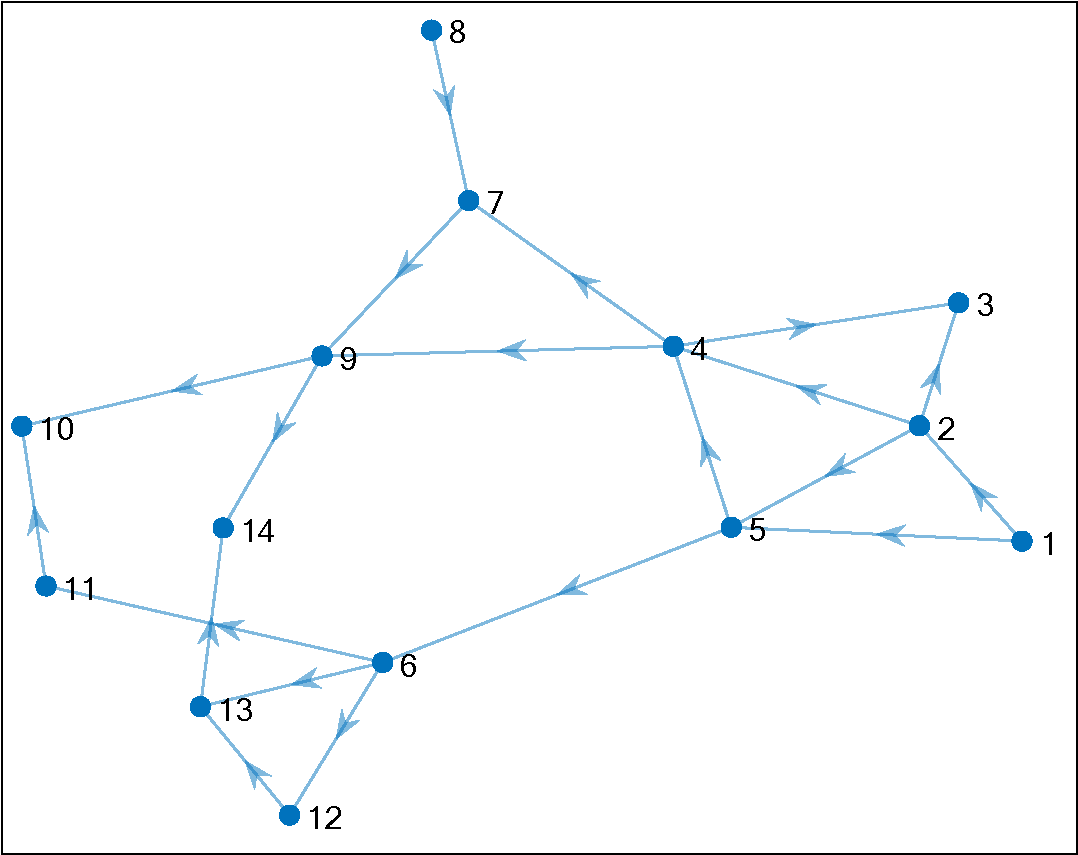
\includegraphics[height=5.8cm]{disgraph14.pdf}
  \caption{基于$PageRank$的拓扑建模}
  \label{fig:model2}
\end{minipage}
\end{figure}
电气介数与$PangRank$计算结果比较如图\ref{fig:compare_nodePR}。由于两个指标基于的拓扑模型不同,所以计算的结果相差较大。首先分析复杂网络的模型,从图中可以看出,支路的电气介数直接影响到了节点的电气介数,比如$2$、$4$、$5$节点由于与节点相连的支路比较重要而对拓扑具有较大的影响力。而支路的重要是因为$1$、$2$、$3$、$6$是系统中的发电节点,其功率传输分布因子较大,故而电电气阶数较大。而$4$、$5$处于发电和负荷的中间传输点,承担了较大的传输潮流的作用,因此相连的支路的电气介数都较大。$8$由于发电功率几乎为零且所连支路只有一条所以电气节数很小。而$12$、$11$、$10$负荷节点相连的支路都不是主要输送支路,功率传输因子小,所以电气节数较小。

反观$PangRank$的模型,该模型将每个节点的重要性赋予在该节点指向其他节点的出链上,因此,那些入链累计度高的节点重要性也高。比如$14$、$10$、$9$,这些节点均是负荷节点,能量最后传输给负荷,由于被潮流指向的累计的节点较多,即该节点的入链节点的入链节点数较多,因此重要性的权重被累计、叠加的程度较大。这种模型也符合现实,实际情况中,能量被输送、汇集到负荷节点,而负荷节点直接与用户相连,直接影响配电质量。因此,负荷节点在结构中的重要性非常高。在$PangRank$的模型中,由于发电节点是潮流起始点,$1$、$8$节点不仅是发电节点,而且是单向输出,没有其他入链,所以其$PR$值较小。

综上分析,电气介数与$PangRank$均对电力系统的结构特点进行了描述,均反映了各个节点在拓扑中的重要程度:前者从能量传输分布的角度对系统的拓扑进行了研究,后者从潮流累计分布的角度对拓扑进行了分析。因此,本文在第四章中将这两个指标进行了融合分析,作为结构脆弱性的综合评价指标。

\begin{figure}[H] % use float package if you want it here
  \centering
  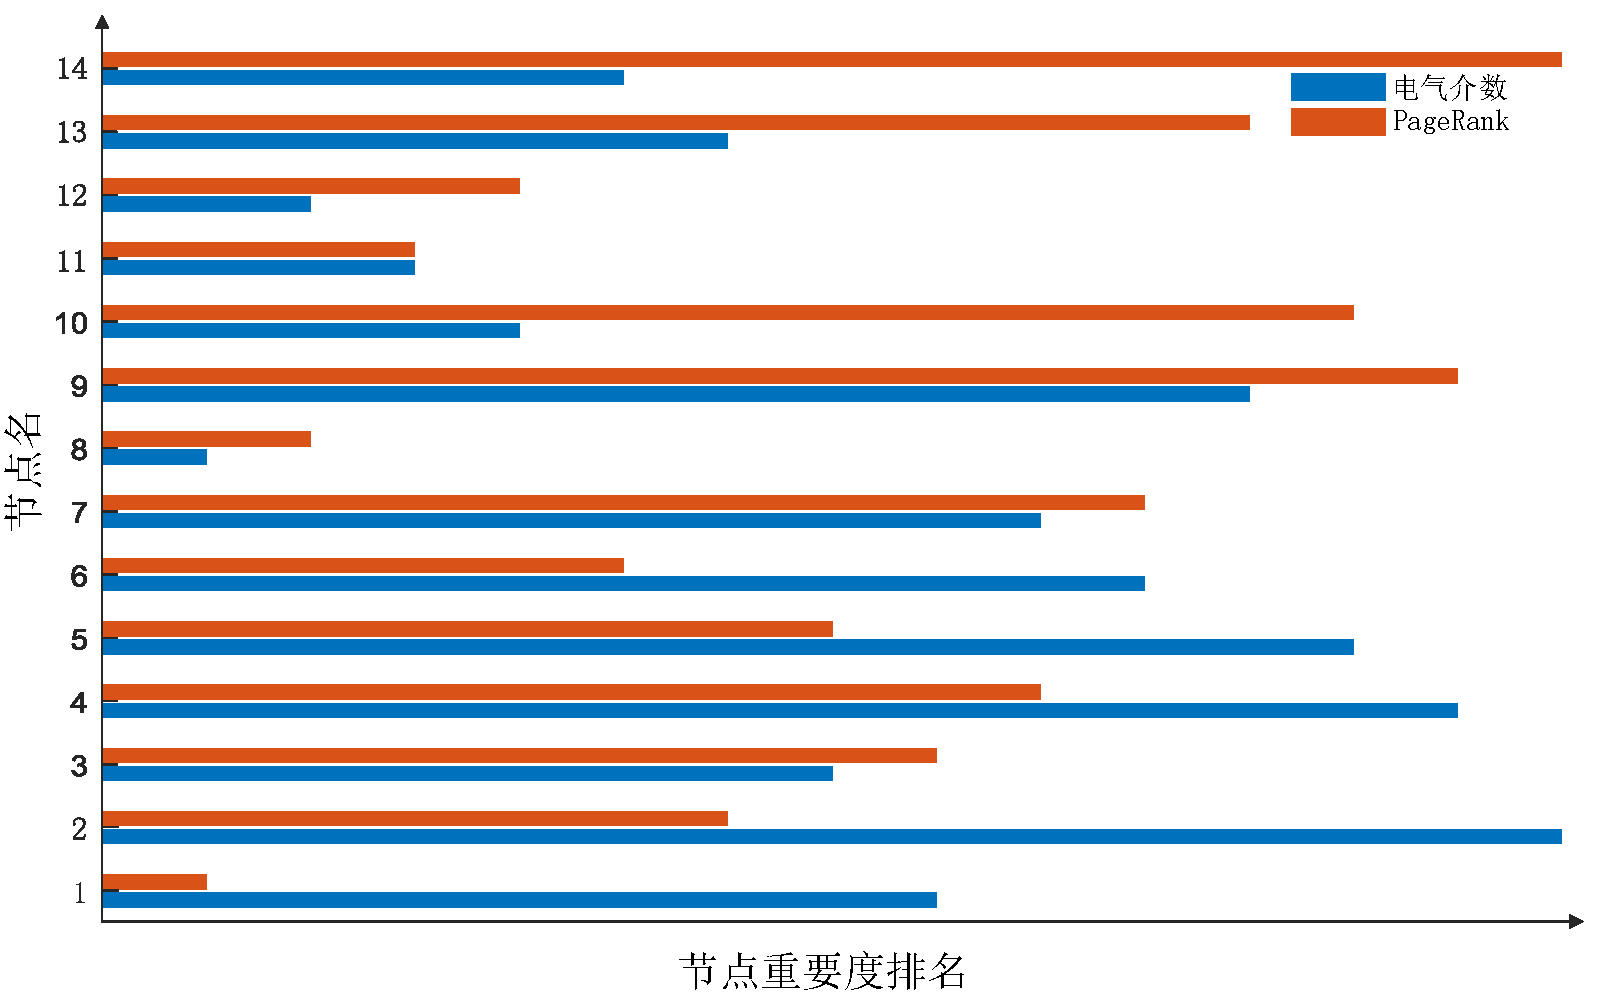
\includegraphics[height=8.7cm]{compare_nodePR.pdf}
  \caption{电气介数与$PangRank$计算结果比较图}
  \label{fig:compare_nodePR}
\end{figure}

\section{电力系统状态脆弱性研究}
\label{sec:status}

电力系统运行中,每个节点或线路都有其对应的状态变量,对电力系统而言,环境的变化会导致系统运行状态变化。环境的变化主要是发电节点容量的变化和负荷节点的负荷容量变化。
因此在电力系统状态研究中,潮流计算扮演了重要的角色。环境的每一次变化都会导致系统的运行状态发生改变,电力系统潮流分布进行重新分配。电力系统的潮流计算是计算每一种
运行状态下系统的运行参数,如电压、功率和相角等,进而判断各个运行参数是否在安全裕度范围内运行,潮流的分布是否合理是潮流计算的基本目标。


\subsection{电力系统状态脆弱性定义与数学描述}
\label{sec:vulneStaus}

电力系统的状态脆弱性是指系统在受到外界扰动或内部自身故障后,节点或线路的状态变量发生变化,并由初始状态(额定状态)向临界点逼近的特性。表现了某个节点或线路从稳定状态向临界失稳
状态的过渡过程。反映了系统的抗干扰能力。

状态脆弱性研究的是电力系统各状态变量偏离正常运行状态及距离临界状态的程度。电力系统的状态量包括功率、电压、相角等。分析方法与传统的稳定性分析方法比较接近,数学描述下:
\begin{equation}
\Delta \alpha=\left|\alpha(t)-\alpha\left(t_{0}\right)\right|  
\end{equation}

式中:$\alpha(t)$表示节点或线路状态变量当前值,$\alpha\left(t_{0}\right)$表示节点或线路状态变量初始值(额定值),$\Delta \alpha$表示当前状态值相较于初始状态值的偏离程度。
那么可用$\Delta \alpha_i$表示元件$i$的状态偏离程度,那么电力系统各元件的状态偏离矩阵为:$D=\left[\begin{array}{lll}{\Delta \alpha_{1},} & {\Delta \alpha_{2},} & {\Delta \alpha_{3} \cdots \Delta \alpha_{n}}\end{array}\right]$

% \begin{equation}
% D=\left[\begin{array}{lll}{\Delta \alpha_{1},} & {\Delta \alpha_{2},} & {\Delta \alpha_{3} \cdots \Delta \alpha_{n}}\end{array}\right]
% \end{equation}

电力系统元件的状态偏离程度还可用百分比的形式进行表示:
\begin{equation}
  \theta=\left|\frac{\alpha(t)-\alpha\left(t_{0}\right)}{\alpha_{m}(t)-\alpha\left(t_{0}\right)}\right|
  \end{equation}

式中:$\alpha_{m}(t)$为元件状态变量的临界值,$\theta$为状态变量当前与初始稳态值的差值与临界偏差量的百分比,它表示状态的变化量相对于临界偏差的偏离程度。当$\theta<1$时,表示
元件处于正常运行状态;当$\Theta>1$时,表示元件偏离临界值,元件处于失稳状态。那么电力系统各元件状态的变化量相对于临界偏差量偏离矩阵为:$E=\left[\begin{array}{lll}{\theta_{1},} & {\theta_{2},} & {\theta_{3} \cdots \theta_{n}}\end{array}\right]$

定义$f\left(\alpha_{1}, \alpha_{2}, \alpha_{3} \cdots \alpha_{n}\right)$为节点$i$或线路$i$状态变量当前值的关联函数,某一状态变量变化导致关联函数变化,当节点或线路$i$当前
状态值发生变化,其关联函数相对当前状态值变化的比值可用如下偏导式进行表达:
\begin{equation}
  \varphi=\frac{\partial f}{\partial \alpha_{i}}
  \end{equation}
将$\varphi$定义为状态灵敏度,表示当前状态值的改变对关联函数的影响程度。那么,电力系统各元件的状态灵敏度矩阵为:$F=\left[\begin{array}{lll}{\varphi_{1},} & {\varphi_{2},} & {\varphi_{3} \cdots \varphi_{n}}\end{array}\right]$

状态脆弱性的数学表达式:
  \begin{equation}
  \left\{\begin{array}{l}{\Delta \alpha=\left|\alpha(t)-\alpha\left(t_{0}\right)\right|} \\
   {\theta=\left|\frac{\alpha(t)-\alpha\left(t_{0}\right)}{\alpha_{m}(t)-\alpha\left(t_{0}\right)}\right|} \\
   {\varphi=\frac{\partial f}{\partial \alpha_{i}}}\end{array}\right.
  \end{equation}
  
系统各元件的矩阵形式的数学表达式:
\begin{equation}
  \left\{\begin{array}{l}{D=\left[\begin{array}{lll}{\Delta \alpha_{1},} & {\Delta \alpha_{2},} & {\Delta \alpha_{3} \cdots \Delta \alpha_{n}}\end{array}\right]} \\
   {E=\left[\begin{array}{lll}{\theta_{1},} & {\theta_{2},} & {\theta_{3} \cdots \theta_{n}}\end{array}\right]} \\
   {F=\left[\begin{array}{lll}{\varphi_{1},} & {\varphi_{2},} & {\varphi_{3} \cdots \varphi_{n}}\end{array}\right]}\end{array}\right.
  \end{equation}




\subsection{蒙特卡洛方法概述}
\label{sec:vulneStaus}






\subsection{负荷模型的建立}
\label{sec:vulneStaus}
结合状态三个指标的模型




\subsection{状态脆弱性分析方法及指标研究}
\label{sec:static}







\section{本章小结}
\label{sec:sum3}





